\documentclass[]{article}
\usepackage[utf8]{inputenc}
\usepackage{natbib}
\usepackage{graphicx}
\usepackage{geometry}
\usepackage{hyperref}






\geometry{
	a4paper,
	total={170mm,257mm},
	left=20mm,
	top=20mm,
}

%opening
\title{Progetto di Algoritmi Avanzati  	
		\\ \large Capacitated Vehicle Routing Problem 
		 \\  Algoritmi: Costruttivi, a 2 Fasi e Genetici}
	 

\author{Giulio Pilotto - Matricola:1140718}

\date{Luglio 2019}

	

\begin{document}
	



\maketitle


\begin{abstract}

Questo elaborato presenta il progetto di Algoritmi Avanzati sottomesso al prof. Bresolin dell'Università di Padova.
Il progetto richiede di implementare almeno 2 algoritmi che risolvono istanze di : Capacitated Vehicle Routing Problem.
Nel seguente elaborato oltre ad implementare i 2 algoritmi richiesti , il primo come metodo costruttivo; Clarke and Wright e il secondo come metodo a 2 fasi:ClusterFirst - Route Second per il quale sono state implementate due tecniche di routing: Nearest-Neighbourn e Dijkastra.
Sono stati implementati altri 2 algoritmi uno che cade sempre nella classe dei metodi a 2 fasi: RouteFirst - ClusterSecond, e un altro che cade nella categoria degli algoritmi metauristici detti anche algoritmi genetici.
Inoltre, è stato implementato un metodo di selezione dei centroidi che tiene conto sia della distanza dal deposito sia della distanza inter-cluster.
Tutti gli algoritmi sono stati testati sulle 16 istanze fornite dalla libreria TSPLIB95.
I risultati confermano che a fronte di una minore accuratezza di una soluzione rispetto all'ottimo ma una maggiore richiesta di risorse in termini di tempo, possono portare a soluzioni ben approssimate.
In particolare scegliere i centrodi con il metodo RadiusRadar permette di guadagnare qualche decimo a fronte di un tempo inore.
Le soluzioni posso essere migliorate attrverso gli algoritmi genetici che fungono da esploratori di uno spazion locale.

\end{abstract}

\section{Introduzione}
Con la nascita dei nuovi servizi per il cliente, che danno assistenza e portao i prodotti direttamente sulla soglia di casa (es:Amazon Prime), la gestione della logistica predilige gran parte degli investimenti.
Questo fatto diventa ancor più importante se diamo un occhiata ai dati forniti dall' Associazione Nazionale Filiera Industria Automobilistica (ANFIA) nel 2017 \ref{fig:ITA28} , dove viene sottolineato che i camion movimentano l'80$\%$ delle merci su terra \cite{ANFIA2017}. 
Gli investimenti non riguardano solo le strutture o gli strumenti fisici, ma soprattutto i software per la gestione e l'ottimizzazione  della distribuzione dei beni.
Grazie all'informatizzazione dei processi da parte del nuovo programma di industrializzazione chiamato "industria 4.0", si può godere di banche dati ricche ed aggiornate, attraverso le quali, possono essere implementate tecniche di ricerca operativa e ottimizzazione.

Il Vehicle Routing Problem \textbf{(VRP)}  è un classe reale di problemi di soddisfacimento di vincoli, in inglese detto anche Constraint Satisfaction Problem \textbf{(COP)}.
Alla fine degli anni cinquanta Dantzig and Ramser hanno formalizzato il problema \cite{dispatching} che riguarda la distribuzione di benzina da un deposito princiapale ad un grande numero di stazioni di servizio.
Da quel momento l'interesse nei problemi VRP è evoluto da un piccolo gruppo di matematici ad un grande gruppo di ricercatori da differenti discipline ancora oggi coinvolti.


VRP consiste nell'ottimizzare l'uso di un insieme di veicoli per prelevare della merce da uno o più depositi e consegnarle presso dei clienti che richiedono una certa quantità di merce.
Le stazioni , i depositi sono distribuiti in uno spazio rappresentato da delle distanze. I mezzi si spostano percorrendo tali distanze, che possono essere rappresentate in maniera diversa.
La maggioranza the problemi reali sono sepsso più complessi del classico VRP. Quindi in pratica VRP è aumentato con dei vincoli, come ad esempio la capacità del veicolo: dove ogni veicolo è caratterizzato da una capacità limitata di carico delle merci, passando quindi da VRP a \textbf{Capacitated - VRP}.
Gli obiettivi sono molteplici:
\begin{itemize}
	\item Minimizzare dei costi di trasporto (istanze percorse, consumo di carburante)
	\item Minimizzare il numero di veicoli
	\item Rispettare il vincolo di capacità imposto  sui veicoli.
	\item Assegnare un percorso ad ogni singolo veicolo.
\end{itemize}


\begin{figure}[h!]
	\centering
	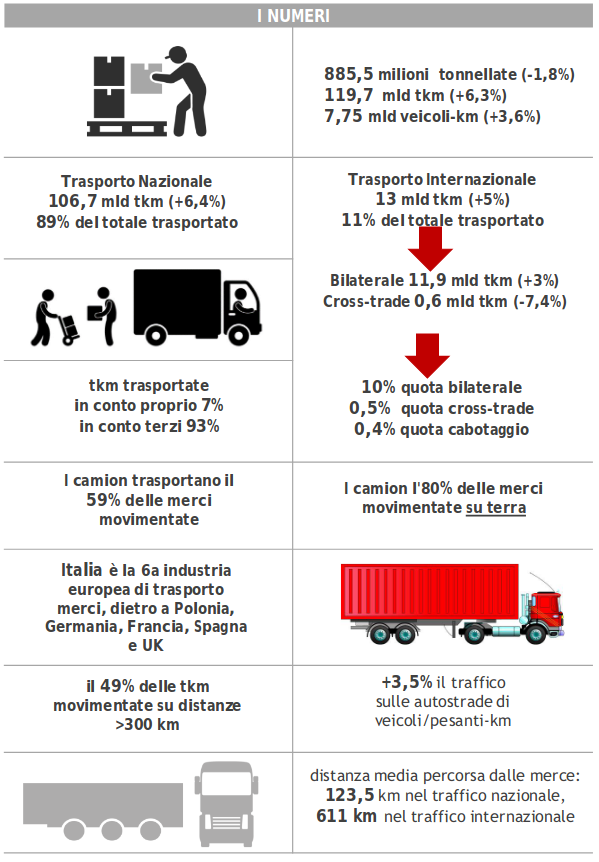
\includegraphics[scale=0.50]{images/ITA28.png}
	\caption{ Italia, traffico merci su strada, ANFIA su dati ISTAT 2017 }
	\label{fig:ITA28}
\end{figure}

VRP è un problema di ottimizzazione combinatoria NP hard,che può essere risolto esattamente trovando l'ottimo solo per piccole istanze del problema. In ogni caso gli approcci euristici che non garantiscono l'ottimalità, forniscono ottimi risultati in pratica.
Negli ultimi 30 anni sono stati applicati anche dei metodi meta-euristici che hanno mostrato una nuova direzione alla ricerca sulla famiglia di problemi VRP.
In questo elaborato vengono prese in esame le istanze fornite dalla libreria TSPLIB95\cite{TSPLIB95}.

Sono stati implementati i seguenti metodi per risolvere le istanze CVRP:
\begin{itemize}
	\item Metodo Costruttivo: Clarke and Wright
	\item Metodo a due fasi:
	\begin{itemize}
		\item Cluster-First Route-Second: Fisher and Jaikumar
		\item Route-First Cluster-Second: Dijkastra
	\end{itemize}
	\item Meta-euristiche: Algoritmi Genetici
\end{itemize}


\section{Related Works}
Quasi tutti i metodi implementati sono euristici perchè nessuno degli algoritmi può garantire di trovare una soluzione ottima per grandi istanze, in un limite di tempo computazionale ragionevole.
Un approccio euristico non esplora l'intero spazio di ricerca, piuttosto cerca di trovare una soluzione basandosi sulle informazioni che ha sul problema.
Le euristiche che risolvono istanze CVRP sono identificati come metodi costruttivi (\textbf{costructive}) e di raggruppamento \textbf{()clustering)}.
I metodi costruttivi costruiscono una soluzione gradualmente,aggiornando continuamente l'informazione che riguarda il costo, ma potrebbe non contenere nessuna fase di miglioramento o di ottimizzazione della soluzione.
Gli algoritmi costruttivi più famosi sono: Clarke and Wright's savings algorithm \cite{CK} , \cite{CK2} , Matching based algorithm e Multi-route improvement heuristic \cite{CK3}.
I metodi di clustering, risolvono il problema in due fasi , ed è per questo che vengono chiamati metodi a 2 fasi.  l'approccio route-first cluster second è caratterizzato dalle due fasi seguenti:
\begin{itemize}
\item \textbf{Fase 1 - Clustering:} Un algoritmo di clustering viene utilizzato per raggruppare i clienti in cluster da dare in pasto alla seconda fase
\item \textbf{Fase 2- Routing} Nella seconda fase, per ogni cluster creato nella prima fase viene ricercata la strada più corta sfruttando tecniche di ottimizzazione.
\end{itemize}
Alcuni famosi algoritmi a due fasi sono: Petal algortihm \cite{petal}, Sweep algorithm \cite{sweep} e Fisher and Jaikumar \cite{FJ}.
Questo studio investiga e compara le performance dei metodi costruttivi e di raggruppamento per risolvere istanze di CVRP.
In particolare, nell'algoritmo di Fisher and Jaikumar, è stato implementato un algoritmo per la selezione dei centroidi chiamato Radar-Radius.Questo  massimizza la distanza tra centroidi (inter-centroid distance) e la distanza tra i centroidi e il deposito in modo da garantire la migliore copertura, a seconda della distribuzione del deposito e dei clienti.
Questo algoritmo è stato implementato scegliendo un deposito per ogni istanza in TSPLIB95,solitamente il deposito con id identificativo 1.
Sono stati usati due metodi diversi per realizzare il routing tra i clienti di uno stesso cluster: Nearest Neighbourn e Dijkastra.



\section{Materiali e Metodi}



\bibliographystyle{unsrt}
\bibliography{biblio}


\end{document}









